\begin{frame}{The Surface of Errors}{Params \#3: $\kappa = 0.5$, $\gamma = 1$, $\rho = -0.9$, $\bar v = 0.04$, $v_0 = 0.04$}
    \begin{figure}
        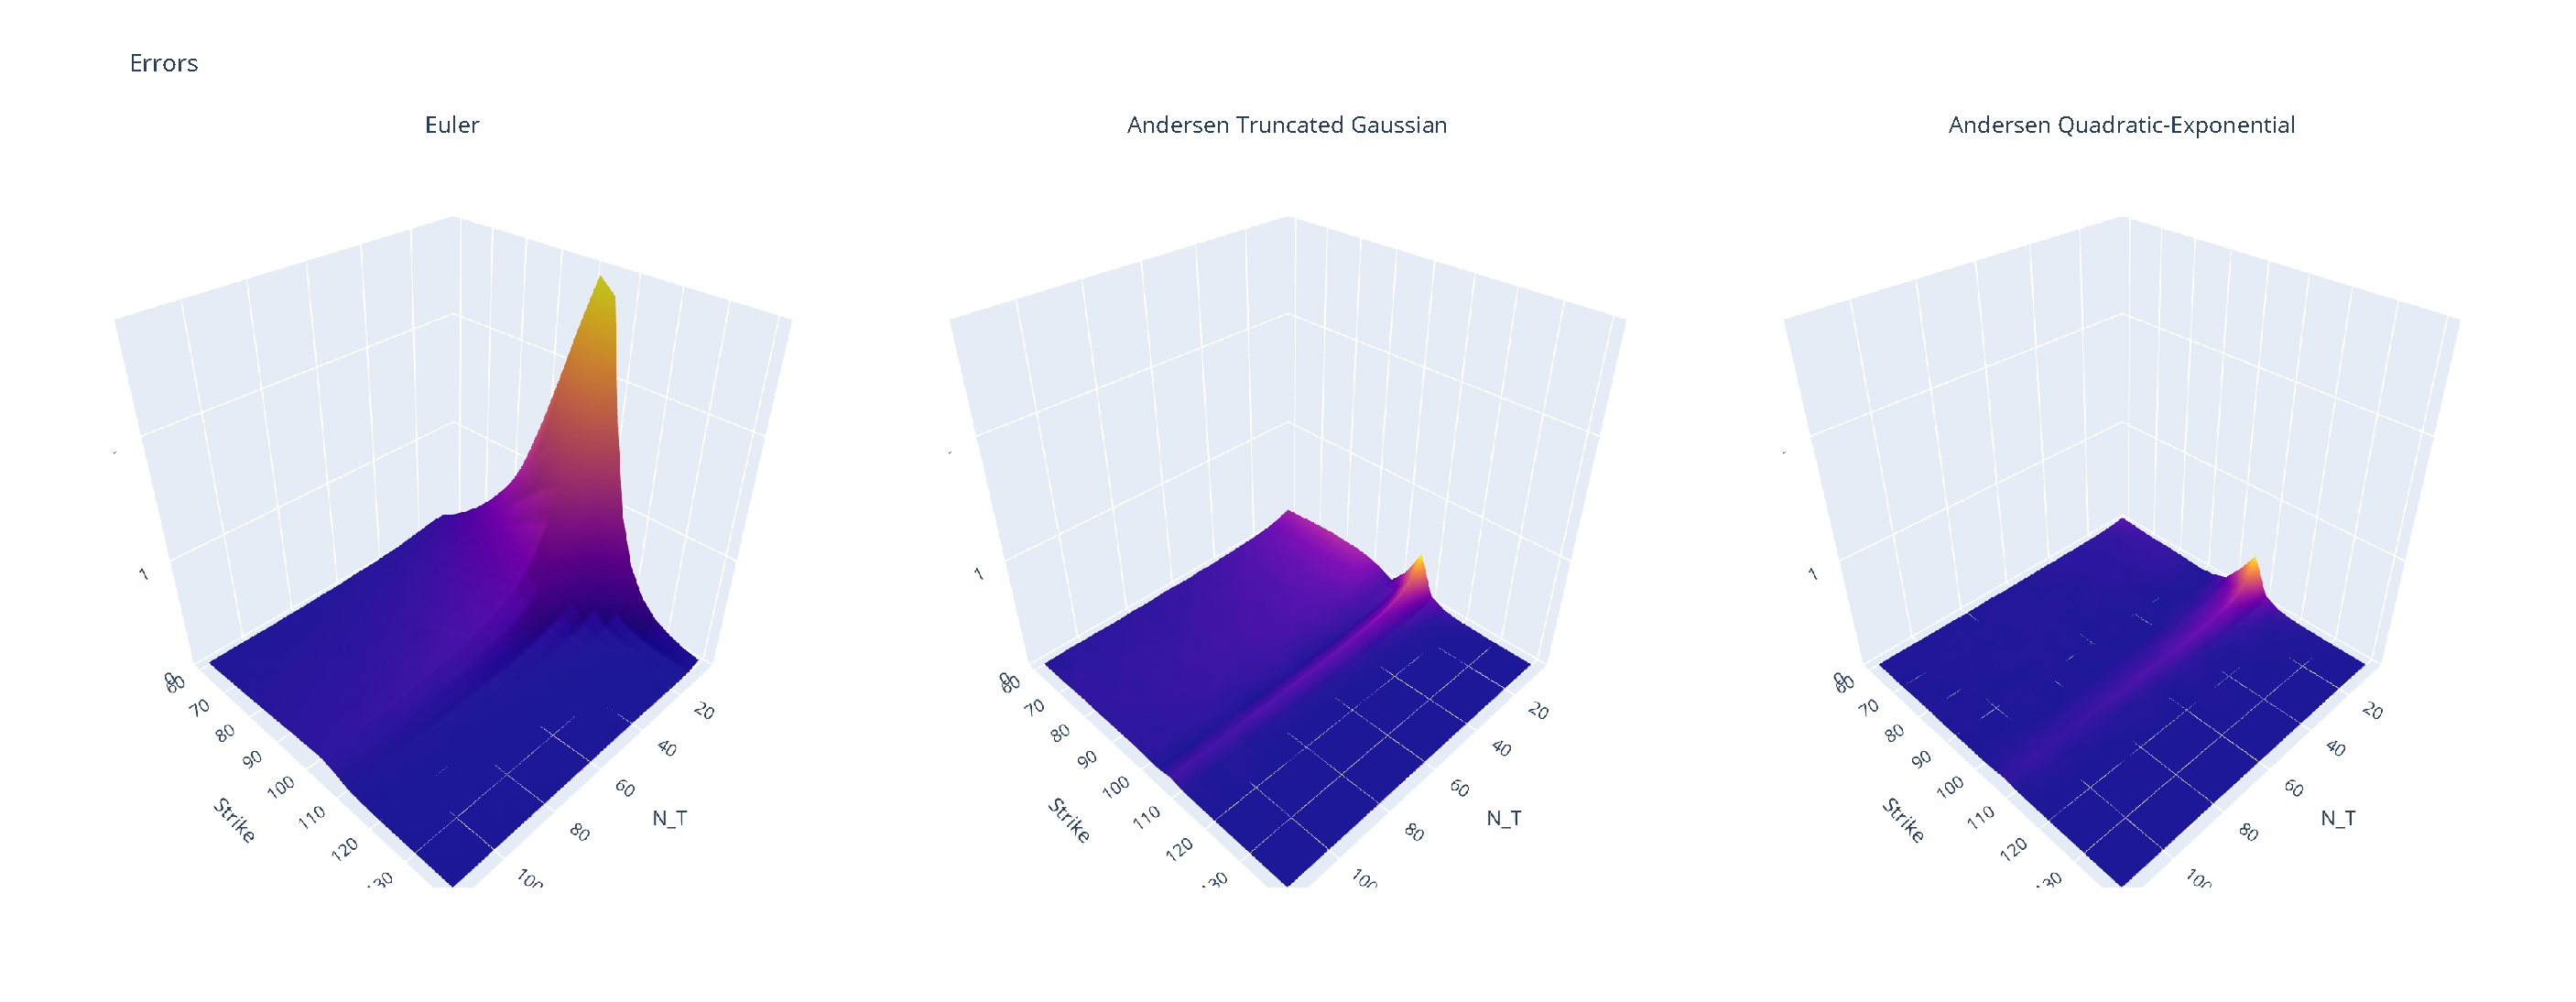
\includegraphics[width=\textwidth]{part4/pictures/err_surface_strike_N_T.pdf}
        \caption{$T=1$, \texttt{absolute\_error = 1e-2}}
    \end{figure}
\end{frame}

\begin{frame}{The Surface of Errors}{Params \#3: $\kappa = 0.5$, $\gamma = 1$, $\rho = -0.9$, $\bar v = 0.04$, $v_0 = 0.04$}
    \begin{table}
    \begin{tabular}{c c c c}
        \hline
        \textbf{Scheme} & \textbf{N\_T} & \textbf{Time} & \textbf{Error}\\
        \hline
        Euler                 &      110      &    1.365      &    0.108692   \\\hline
        Truncated Gaussian    &      10       &    0.131      &    -0.077350  \\
        Truncated Gaussian    &      110      &    1.525      &    -0.002841  \\\hline
        Quadratic-Exponential &      10       &    0.139      &    -0.107819  \\
        Quadratic-Exponential &      110      &    1.590      &    -0.011618  \\
        \hline
        \
    \end{tabular}
    \caption{Accuracy-Performance comparison.}
    \end{table}
\end{frame}

\begin{frame}{The Surface of Errors}{Params \#1: $\kappa = 1.3125$, $\gamma = 0.5125$, $\rho = -0.3937$, $\bar v = 0.0641$, $v_0 = 0.3$}
    \begin{figure}
        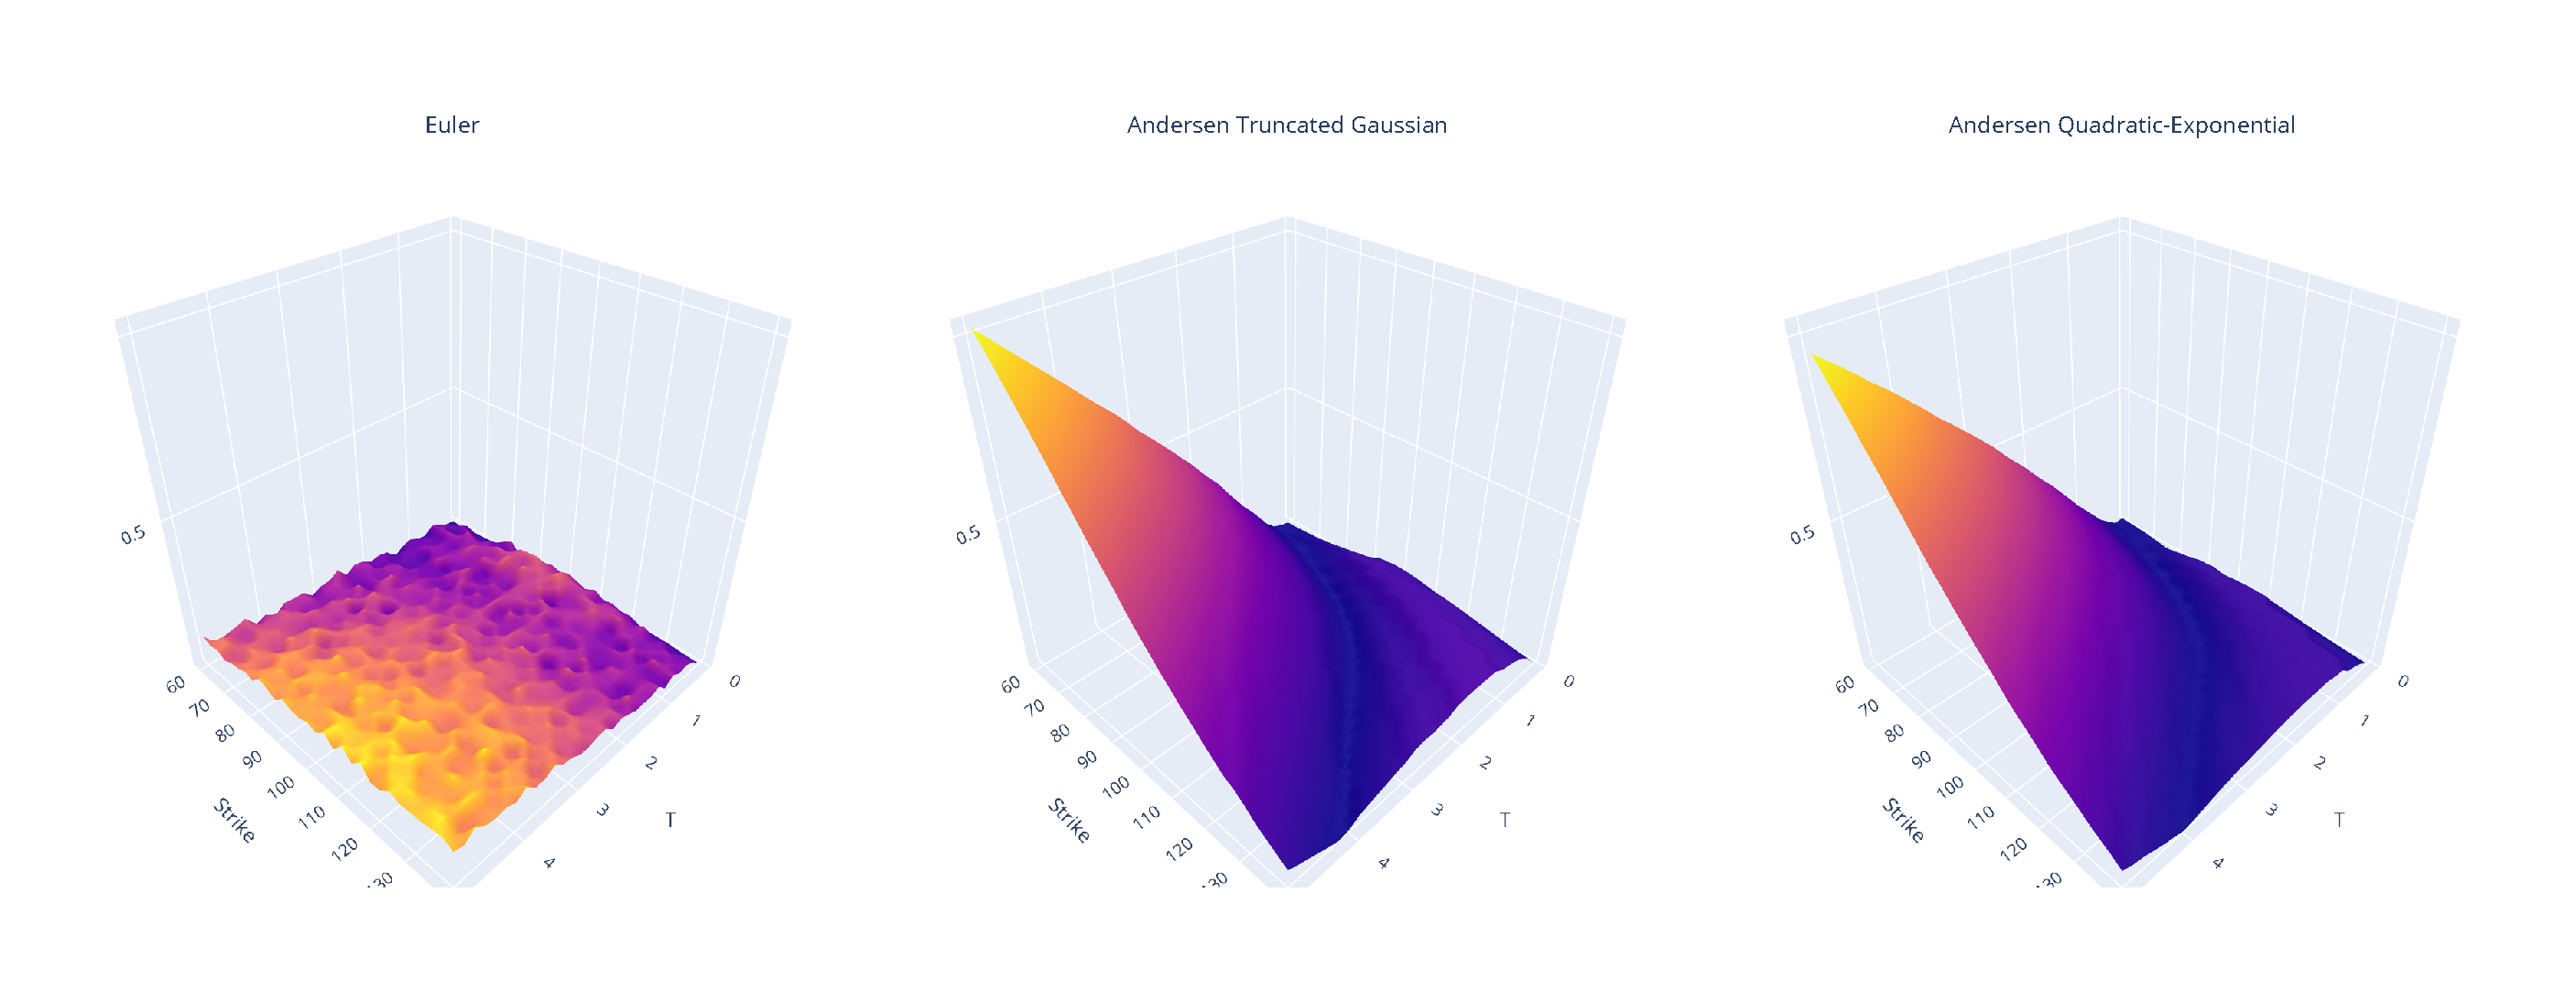
\includegraphics[width=\textwidth]{part4/pictures/err_surface_strike_T_N_T=50_param1.pdf}
        \caption{\texttt{N\_T = 50}, \texttt{absolute\_error = 5e-2}}
    \end{figure}
\end{frame}

\begin{frame}{The Surface of Errors}{Params \#2: $\kappa = 1$, $\gamma = 0.4$, $\rho = -0.1$, $\bar v = 0.2$, $v_0 = 0.2$}
    \begin{figure}
        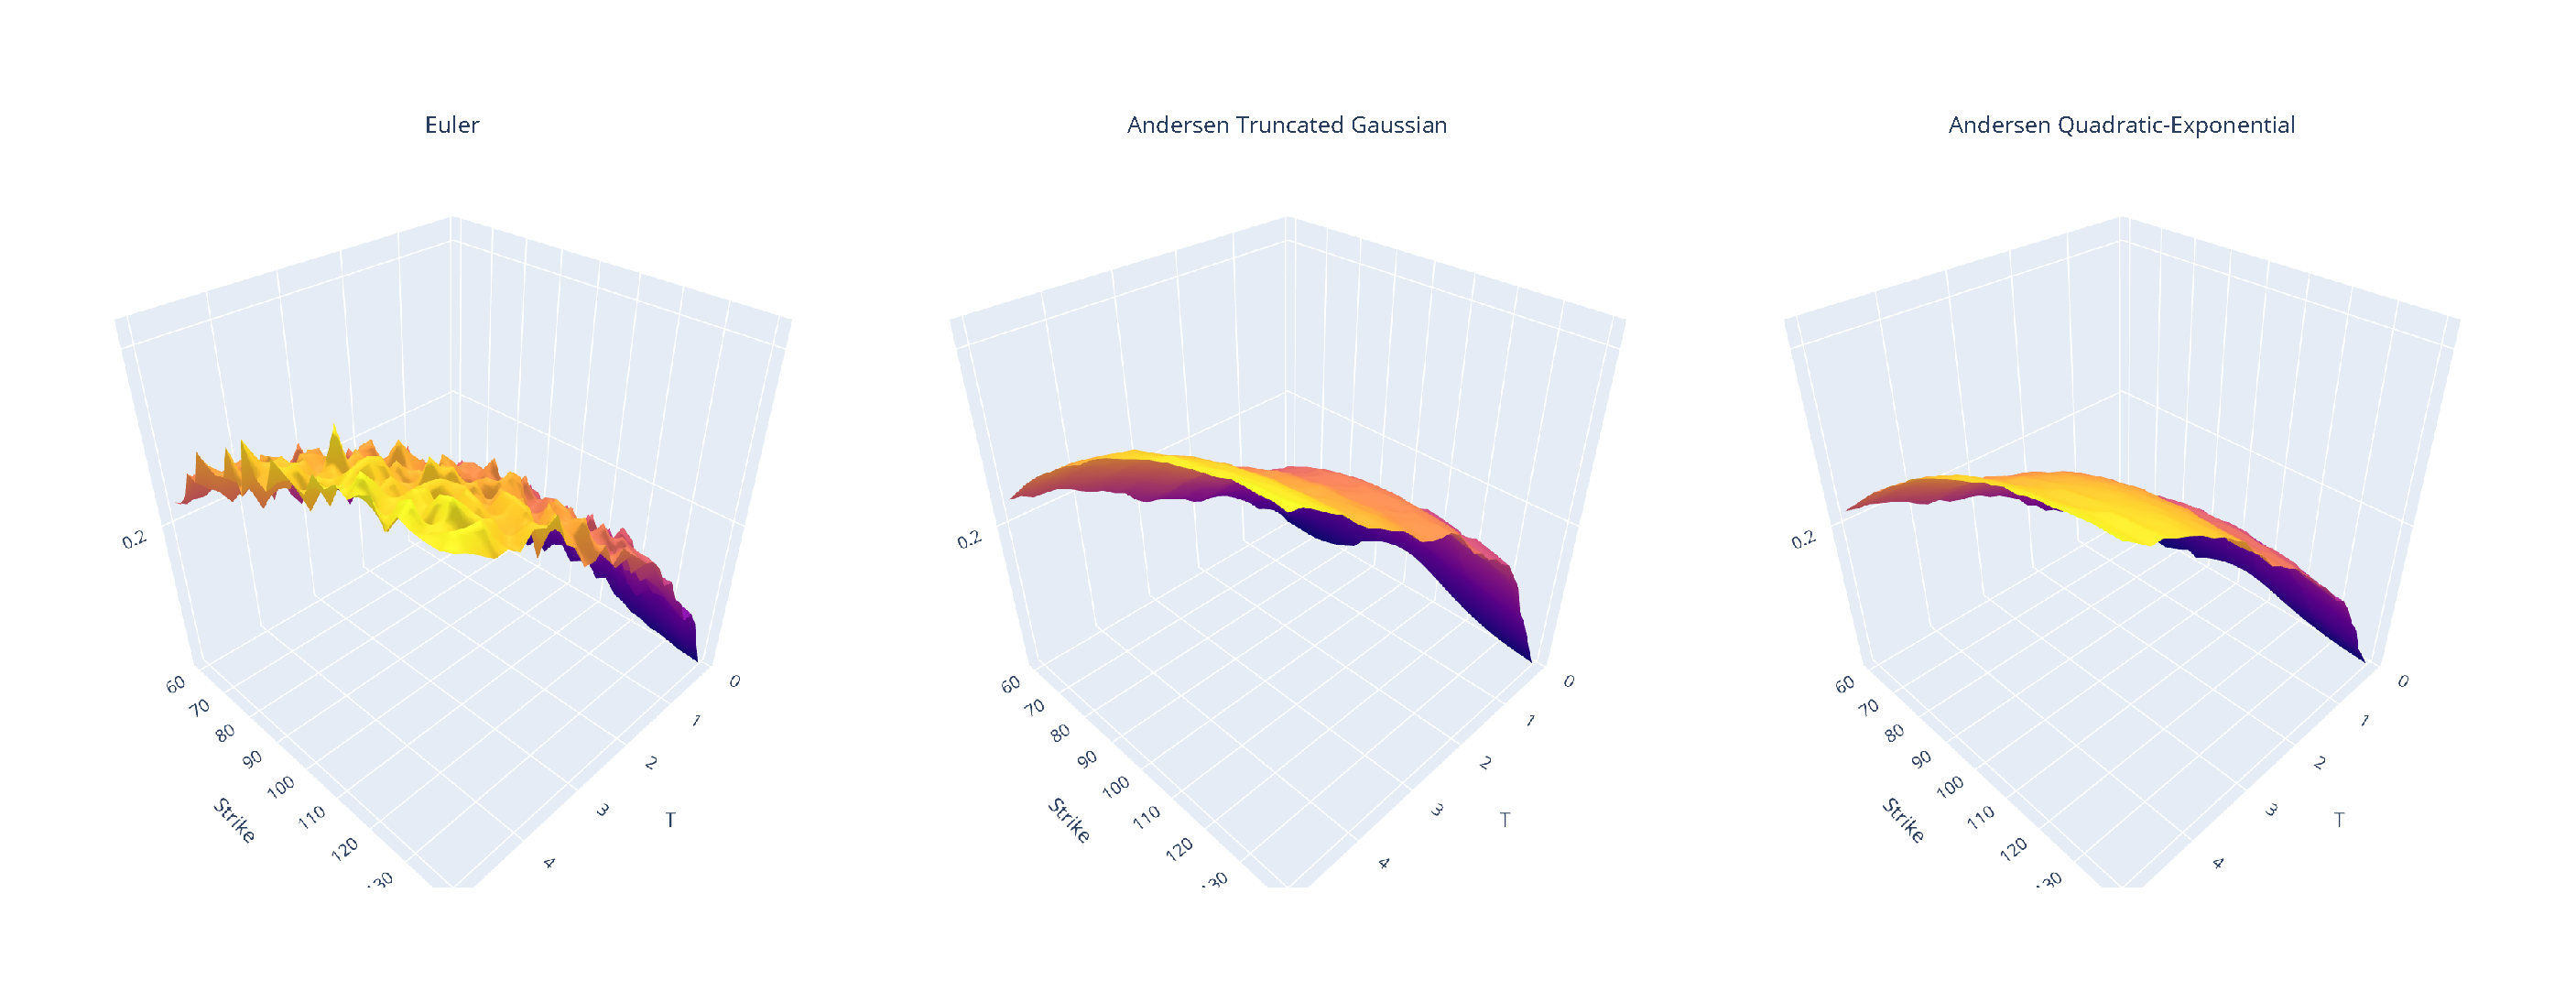
\includegraphics[width=\textwidth]{part4/pictures/err_surface_strike_T_N_T=50_param2.pdf}
        \caption{\texttt{N\_T = 50}, \texttt{absolute\_error = 5e-2}}
    \end{figure}
\end{frame}

\begin{frame}{The Surface of Errors}{Params \#3: $\kappa = 0.5$, $\gamma = 1$, $\rho = -0.9$, $\bar v = 0.04$, $v_0 = 0.04$}
    \begin{figure}
        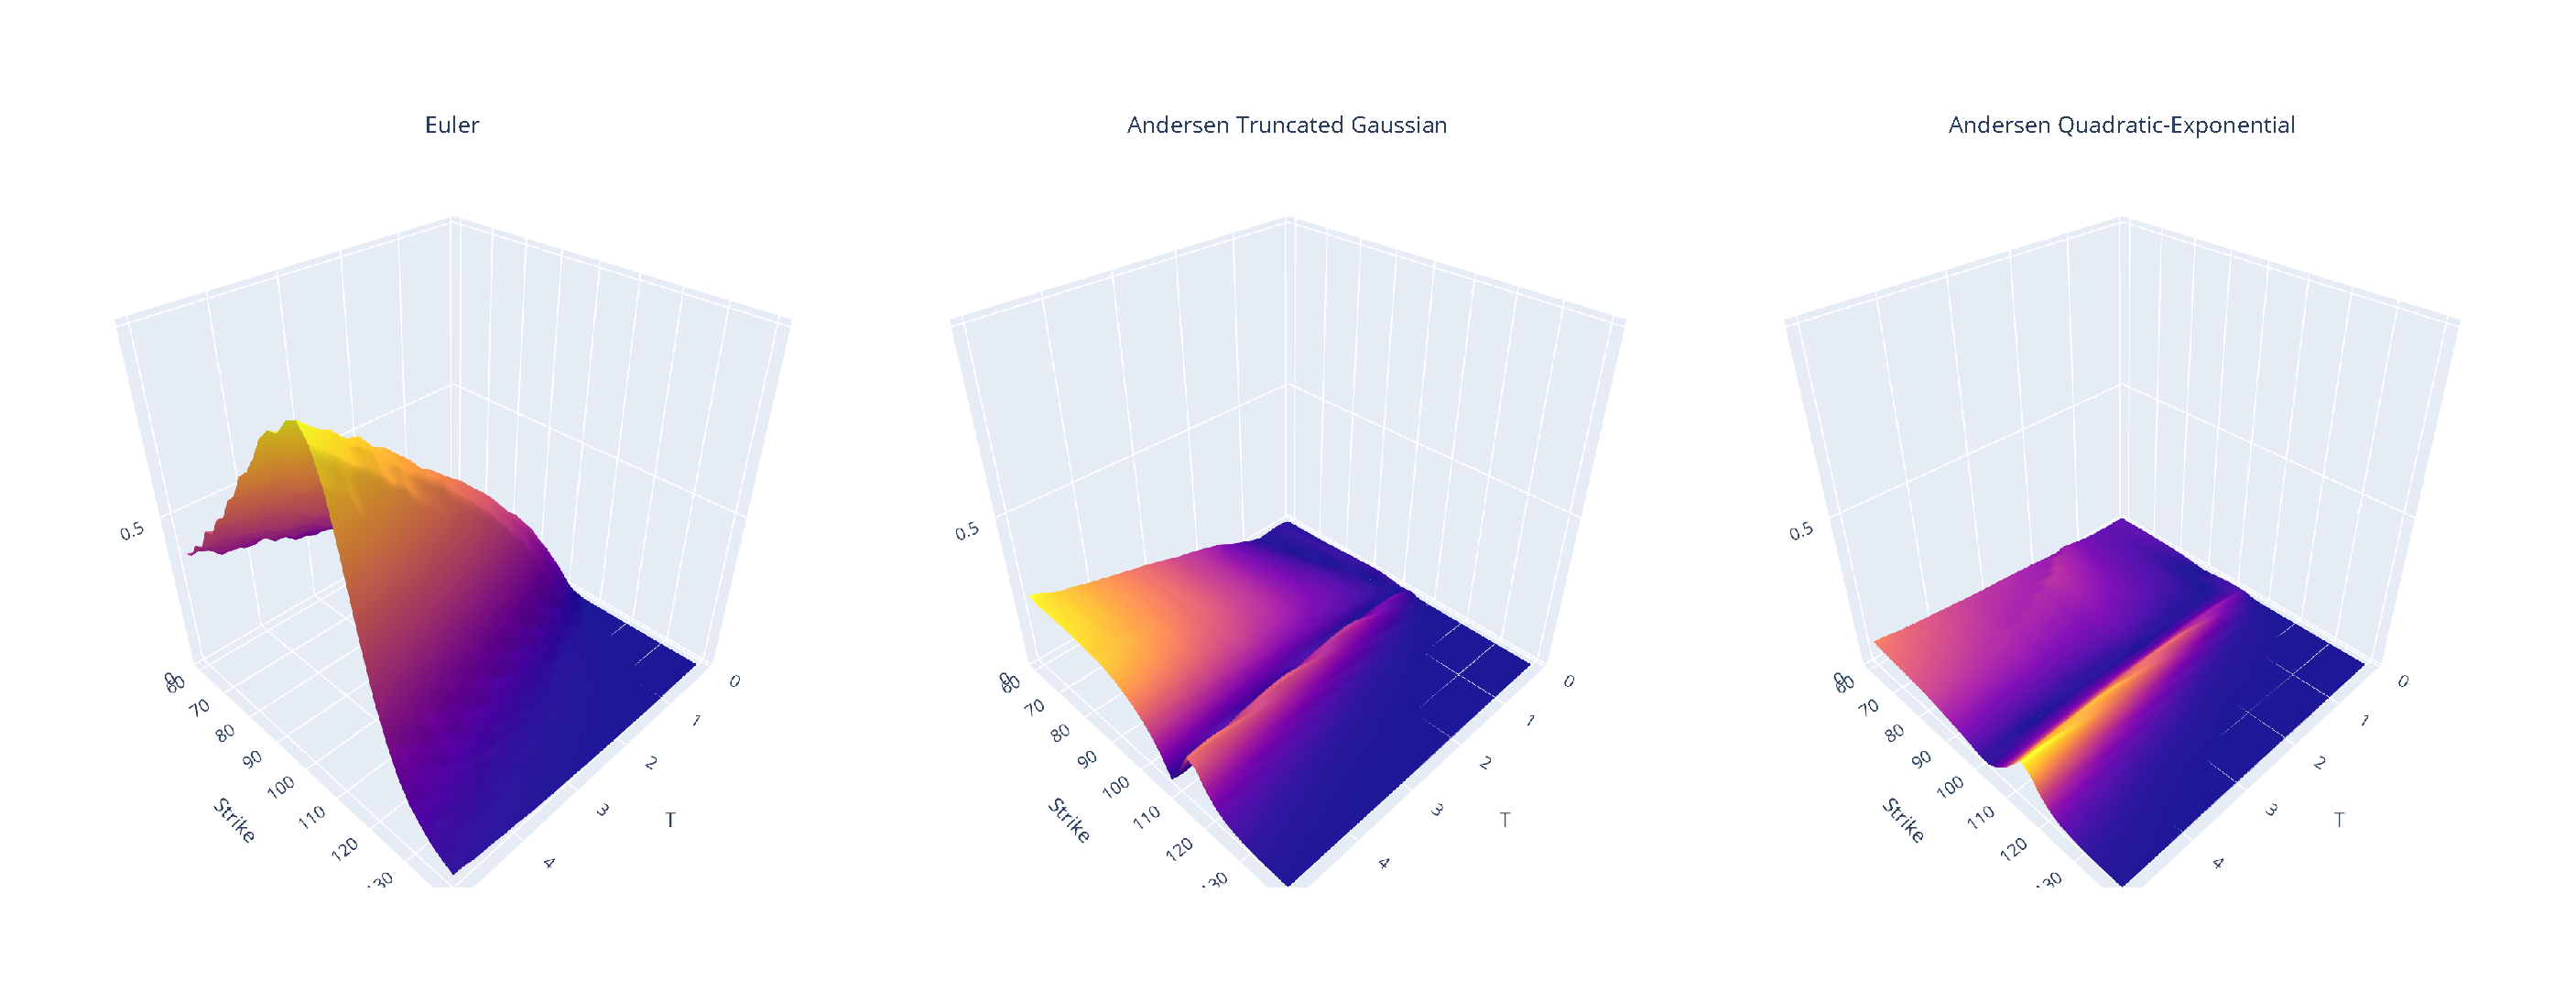
\includegraphics[width=\textwidth]{part4/pictures/err_surface_strike_T_N_T=50_param3.pdf}
        \caption{\texttt{N\_T = 50}, \texttt{absolute\_error = 5e-2}}
    \end{figure}
\end{frame}

\begin{frame}{The Surface of Errors}{Params \#4: $\kappa = 0.3$, $\gamma = 0.9$, $\rho = -0.5$, $\bar v = 0.04$, $v_0 = 0.04$}
    \begin{figure}
        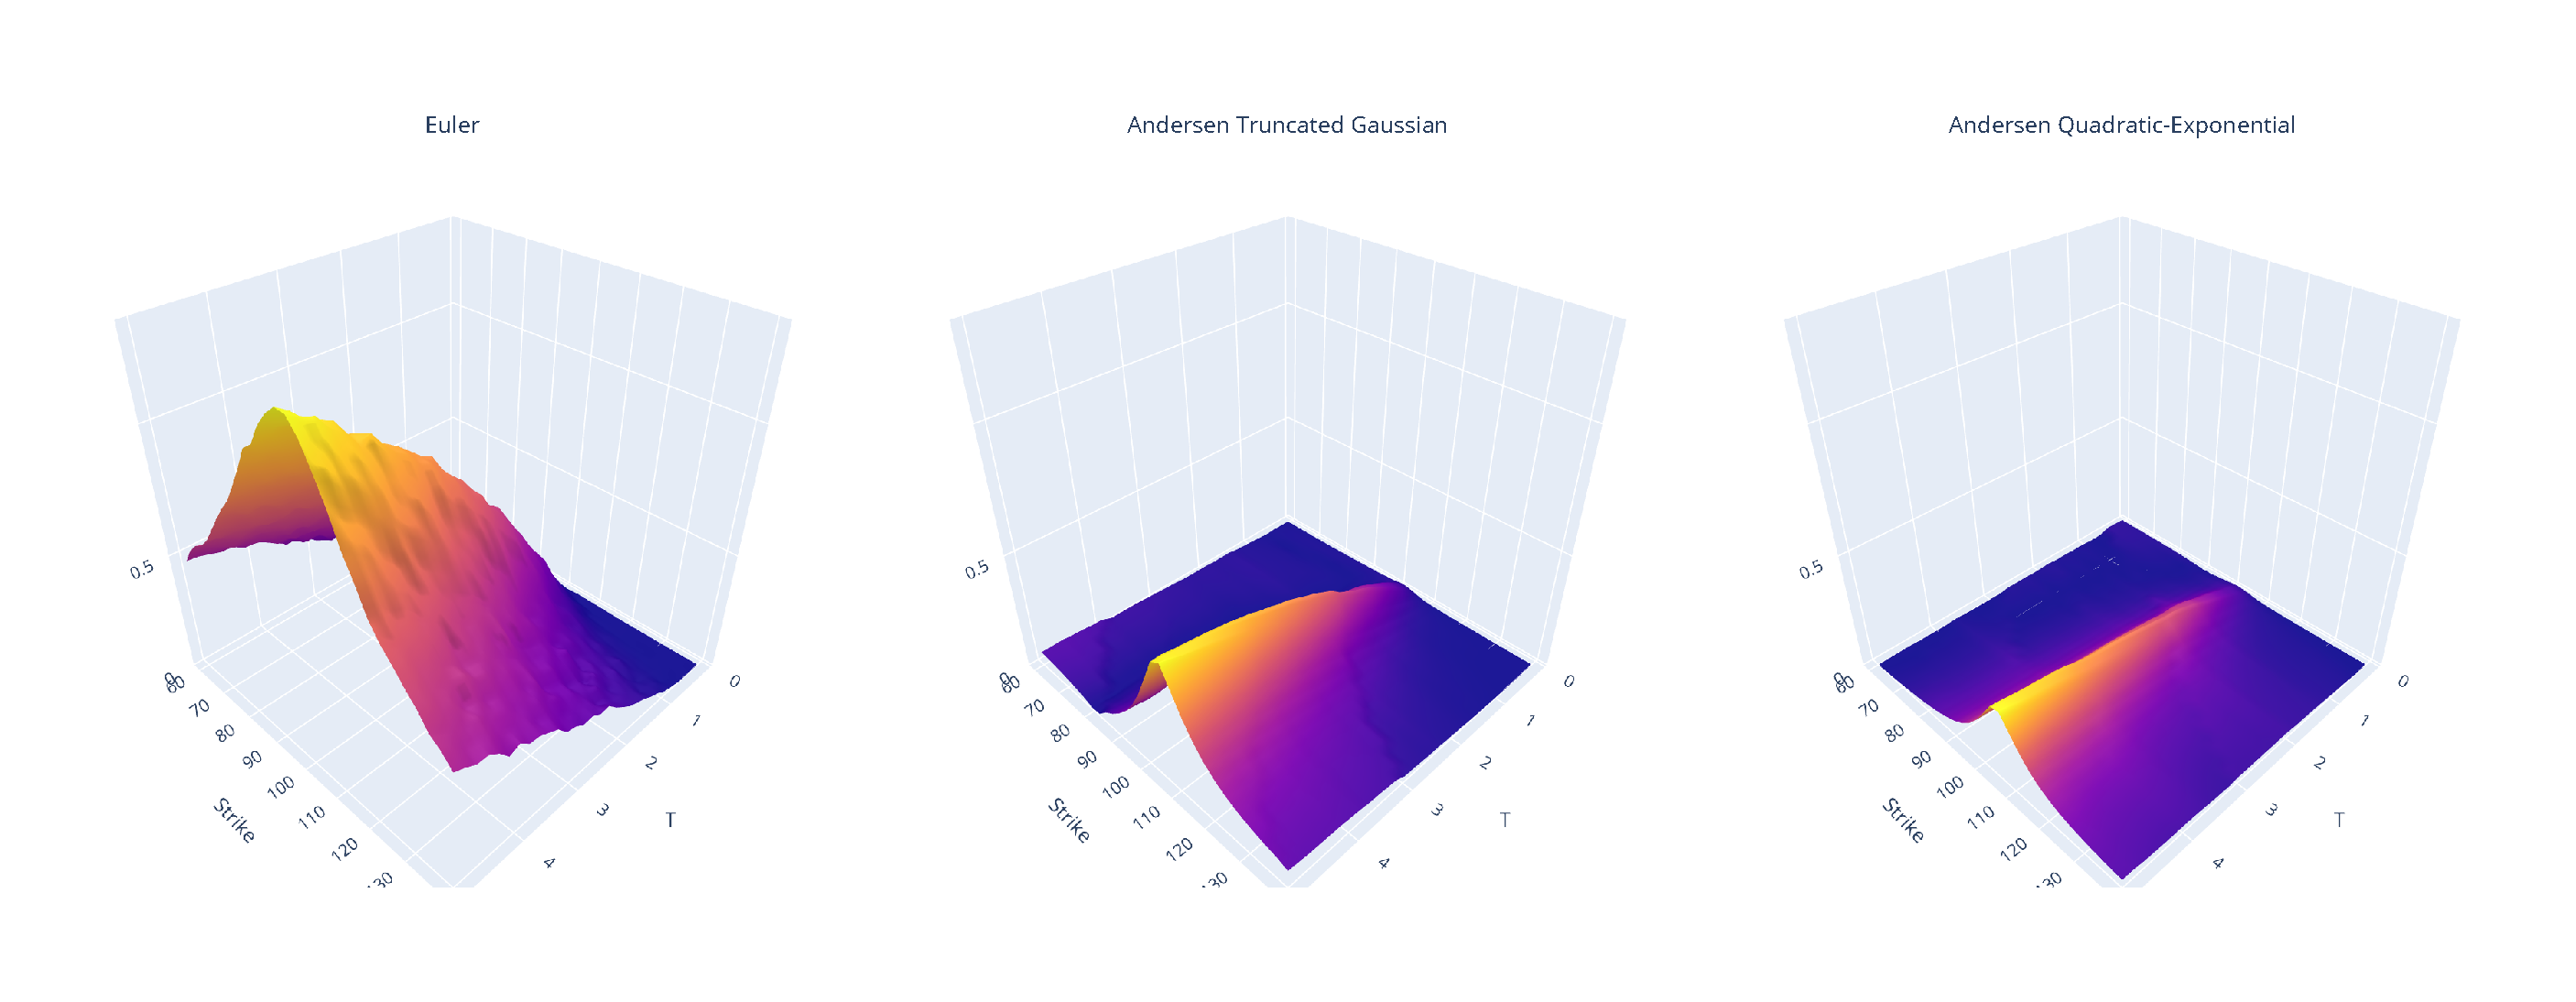
\includegraphics[width=\textwidth]{part4/pictures/err_surface_strike_T_N_T=50_param4.pdf}
        \caption{\texttt{N\_T = 50}, \texttt{absolute\_error = 5e-2}}
    \end{figure}
\end{frame}

\begin{frame}{The Surface of Errors}{Params \#5: $\kappa = 1$, $\gamma = 1$, $\rho = -0.3$, $\bar v = 0.04$, $v_0 = 0.09$}
    \begin{figure}
        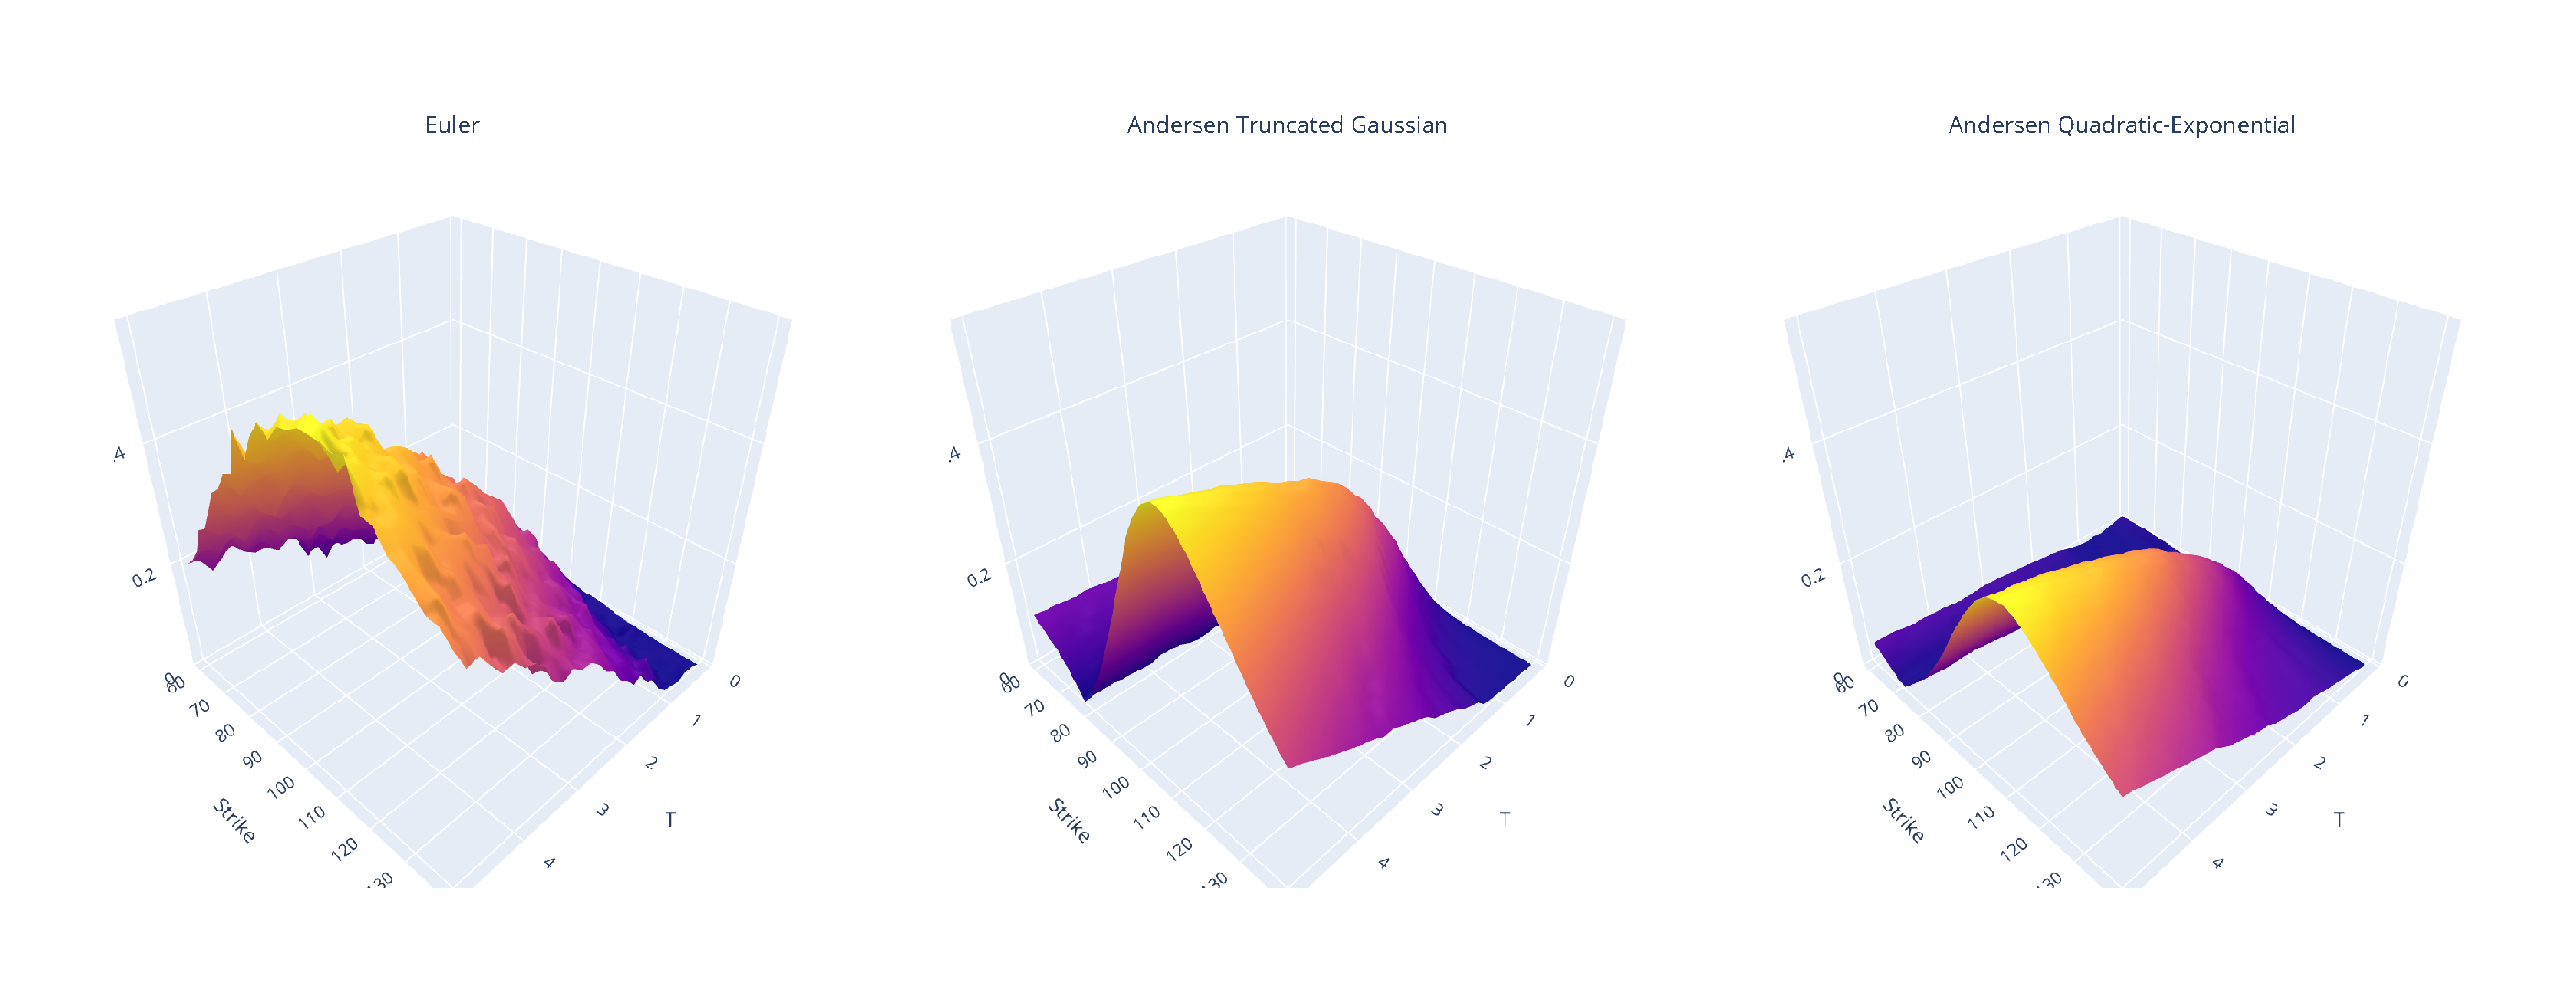
\includegraphics[width=\textwidth]{part4/pictures/err_surface_strike_T_N_T=50_param5.pdf}
        \caption{\texttt{N\_T = 50}, \texttt{absolute\_error = 5e-2}}
    \end{figure}
\end{frame}

\begin{frame}{The Surface of Errors}{Params \#1: $\kappa = 1.3125$, $\gamma = 0.5125$, $\rho = -0.3937$, $\bar v = 0.0641$, $v_0 = 0.3$}
    \begin{figure}
        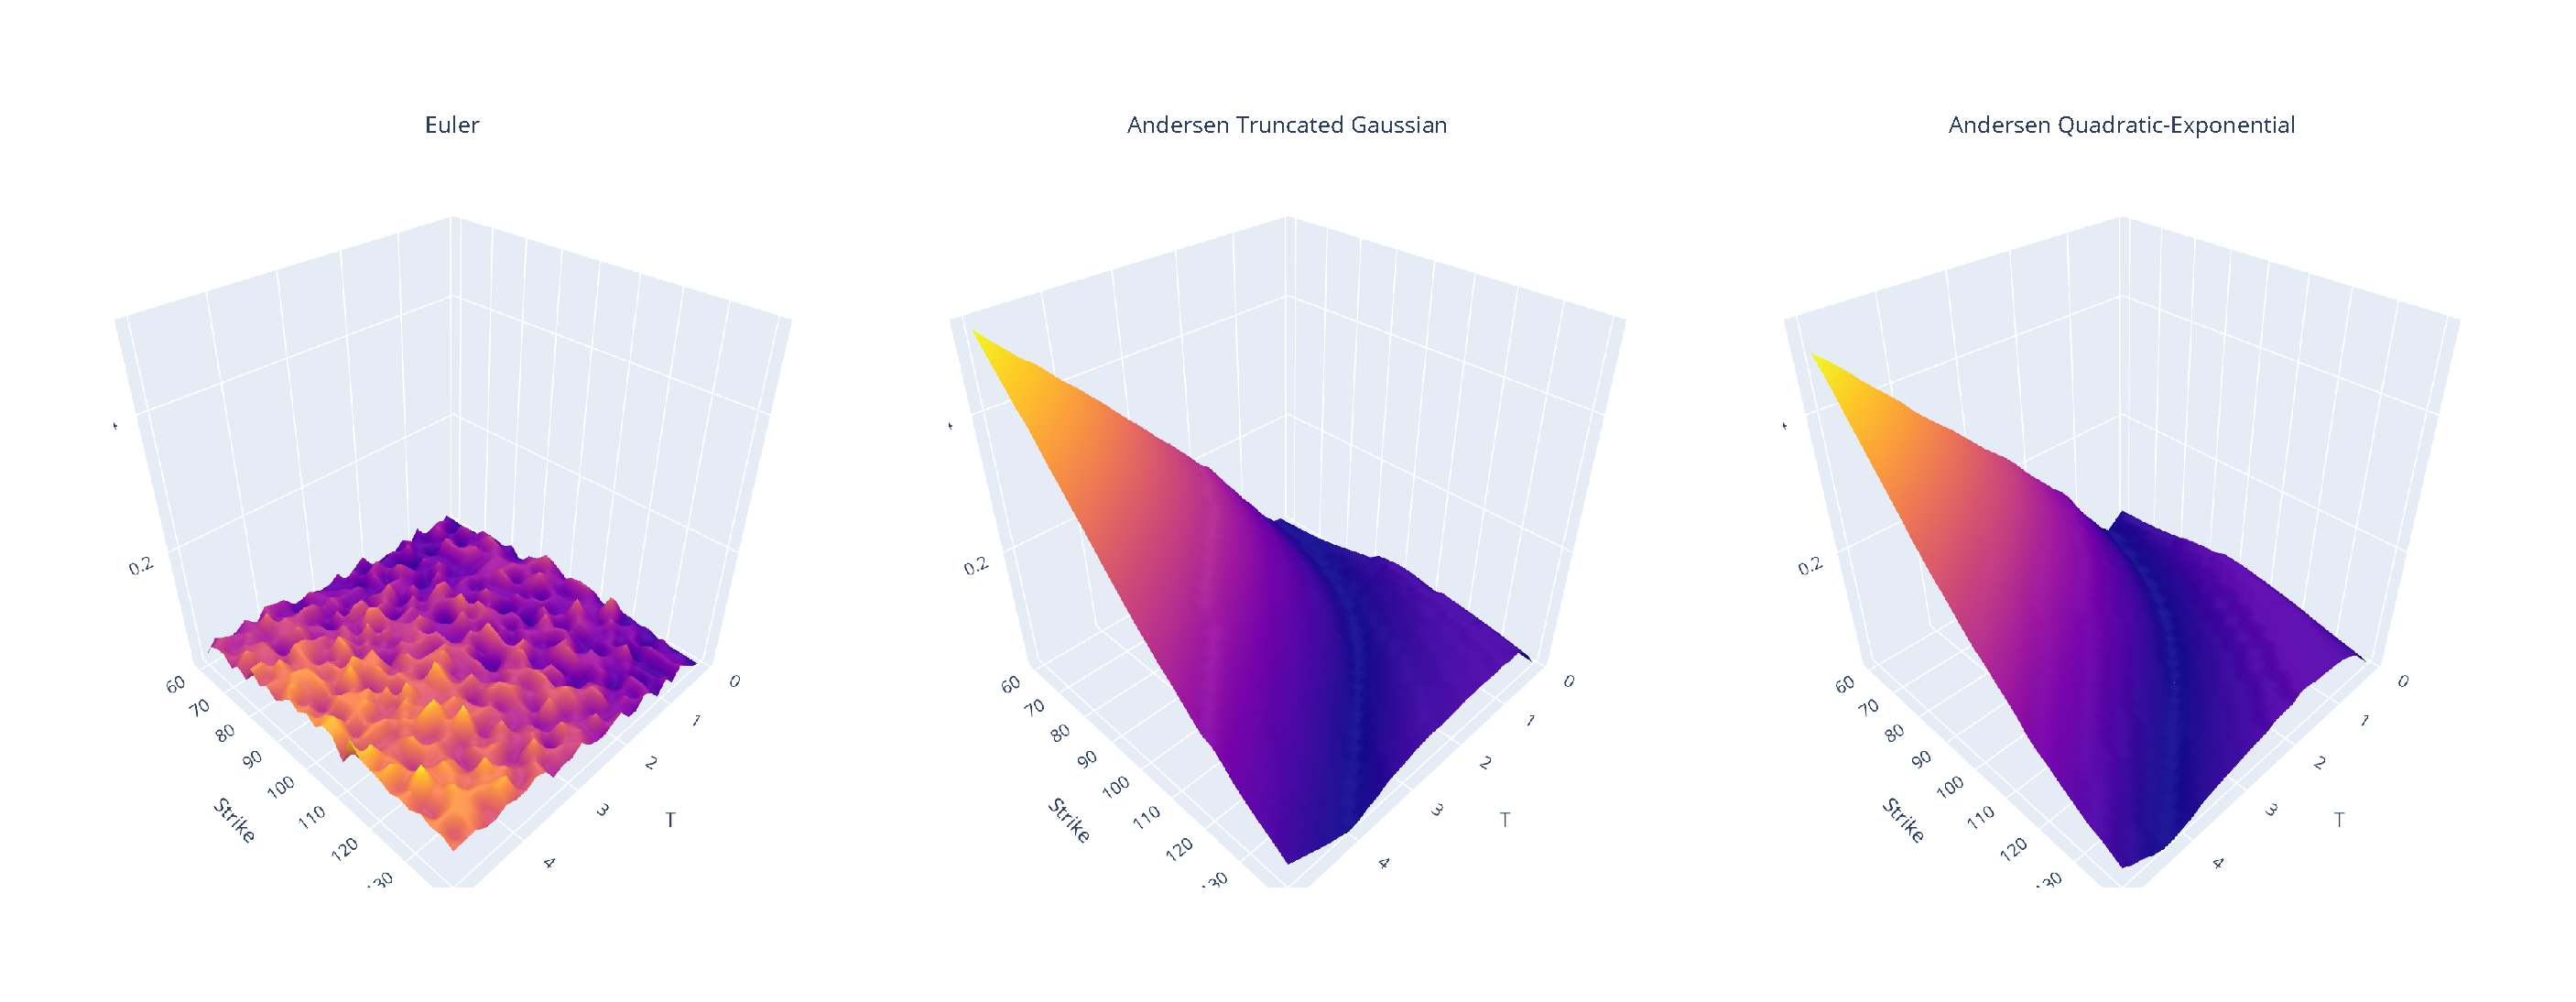
\includegraphics[width=\textwidth]{part4/pictures/err_surface_strike_T_N_T=100_param1.pdf}
        \caption{\texttt{N\_T = 100}, \texttt{absolute\_error = 5e-2}}
    \end{figure}
\end{frame}

\begin{frame}{The Surface of Errors}{Params \#2: $\kappa = 1$, $\gamma = 0.4$, $\rho = -0.1$, $\bar v = 0.2$, $v_0 = 0.2$}
    \begin{figure}
        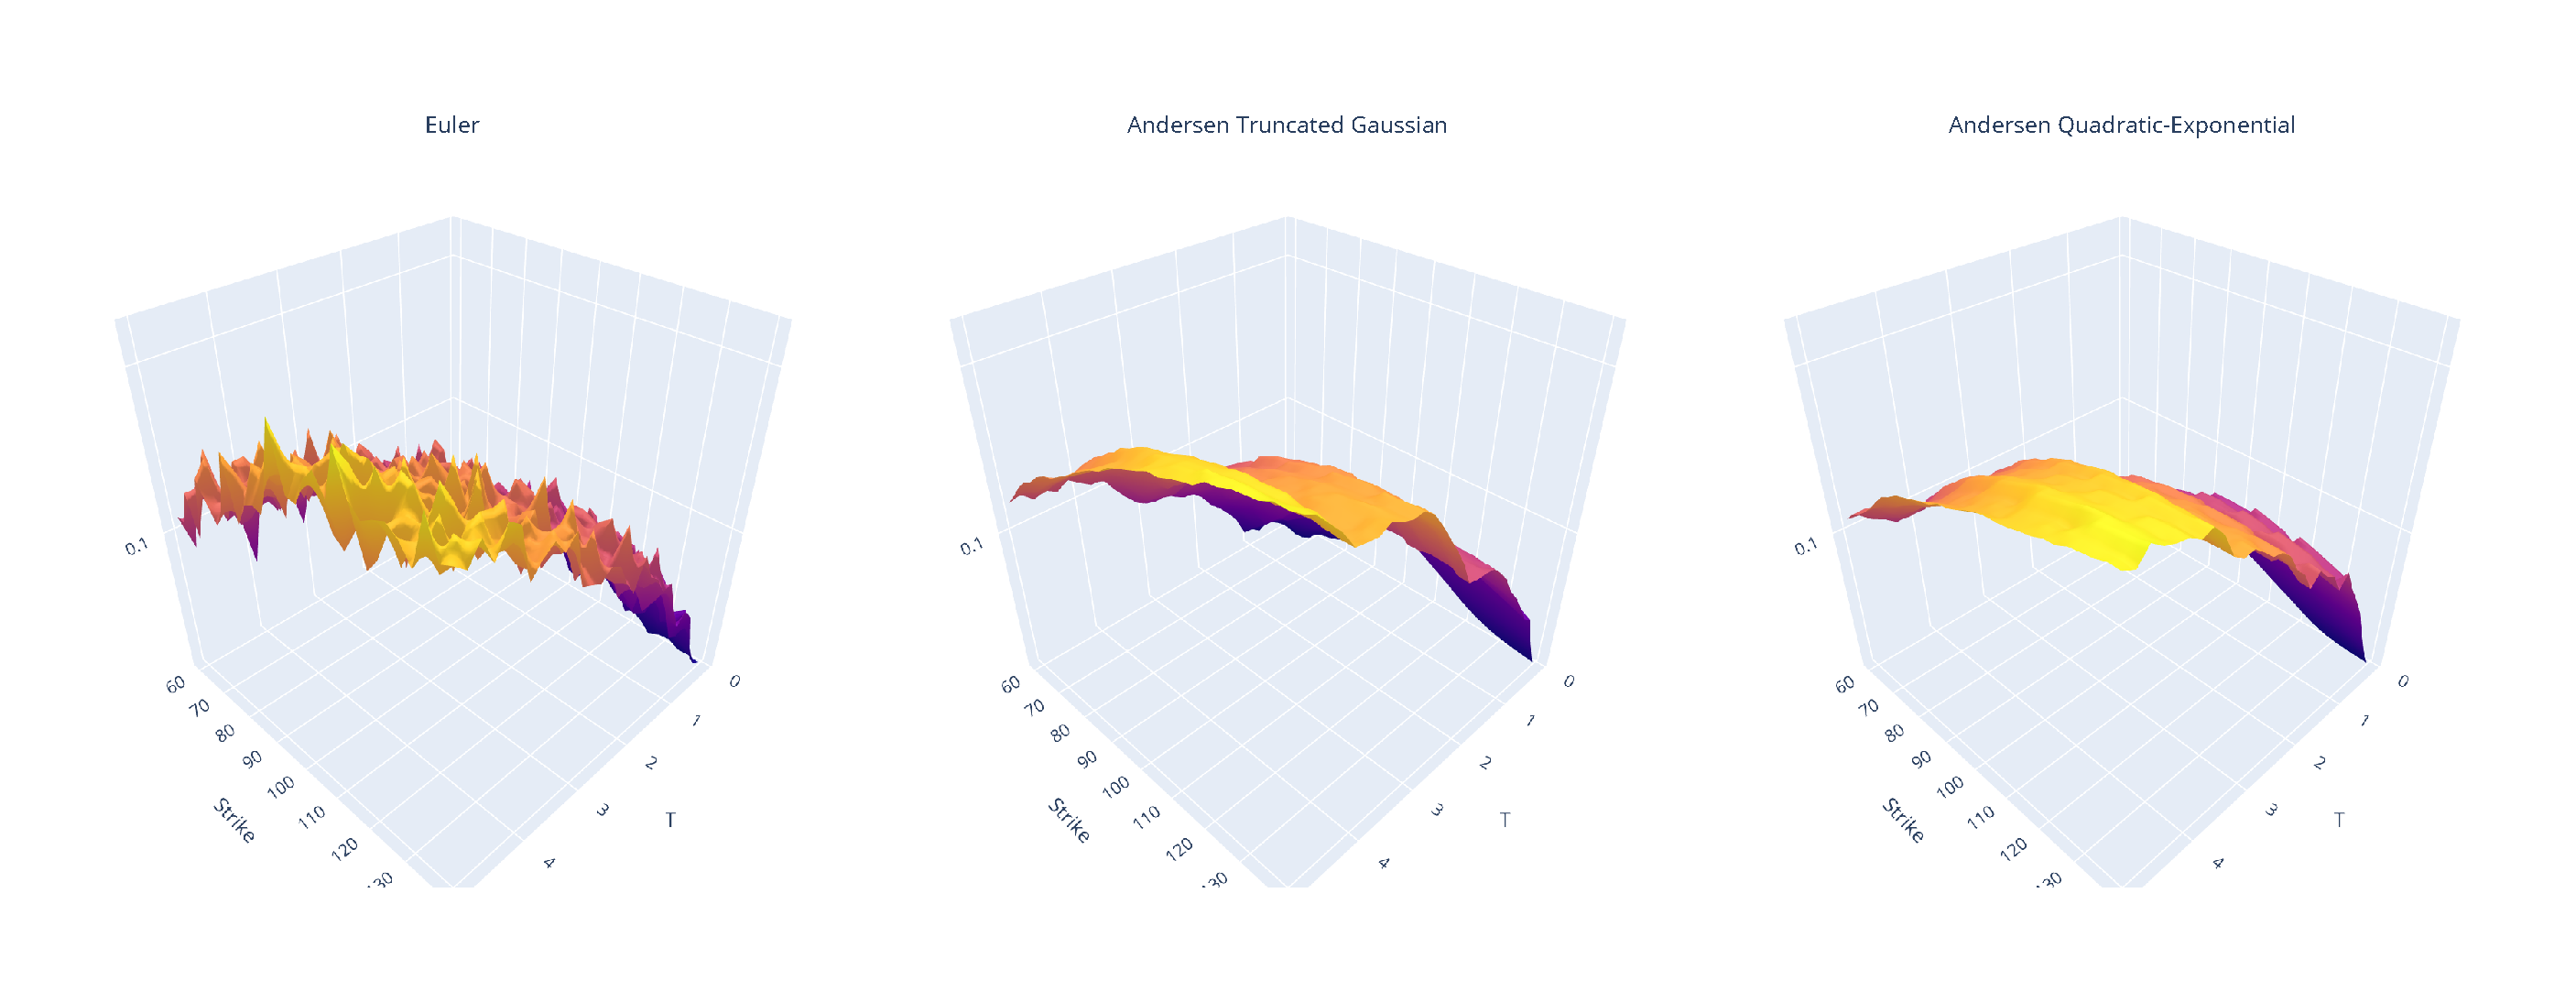
\includegraphics[width=\textwidth]{part4/pictures/err_surface_strike_T_N_T=100_param2.pdf}
        \caption{\texttt{N\_T = 100}, \texttt{absolute\_error = 5e-2}}
    \end{figure}
\end{frame}

\begin{frame}{The Surface of Errors}{Params \#3: $\kappa = 0.5$, $\gamma = 1$, $\rho = -0.9$, $\bar v = 0.04$, $v_0 = 0.04$}
    \begin{figure}
        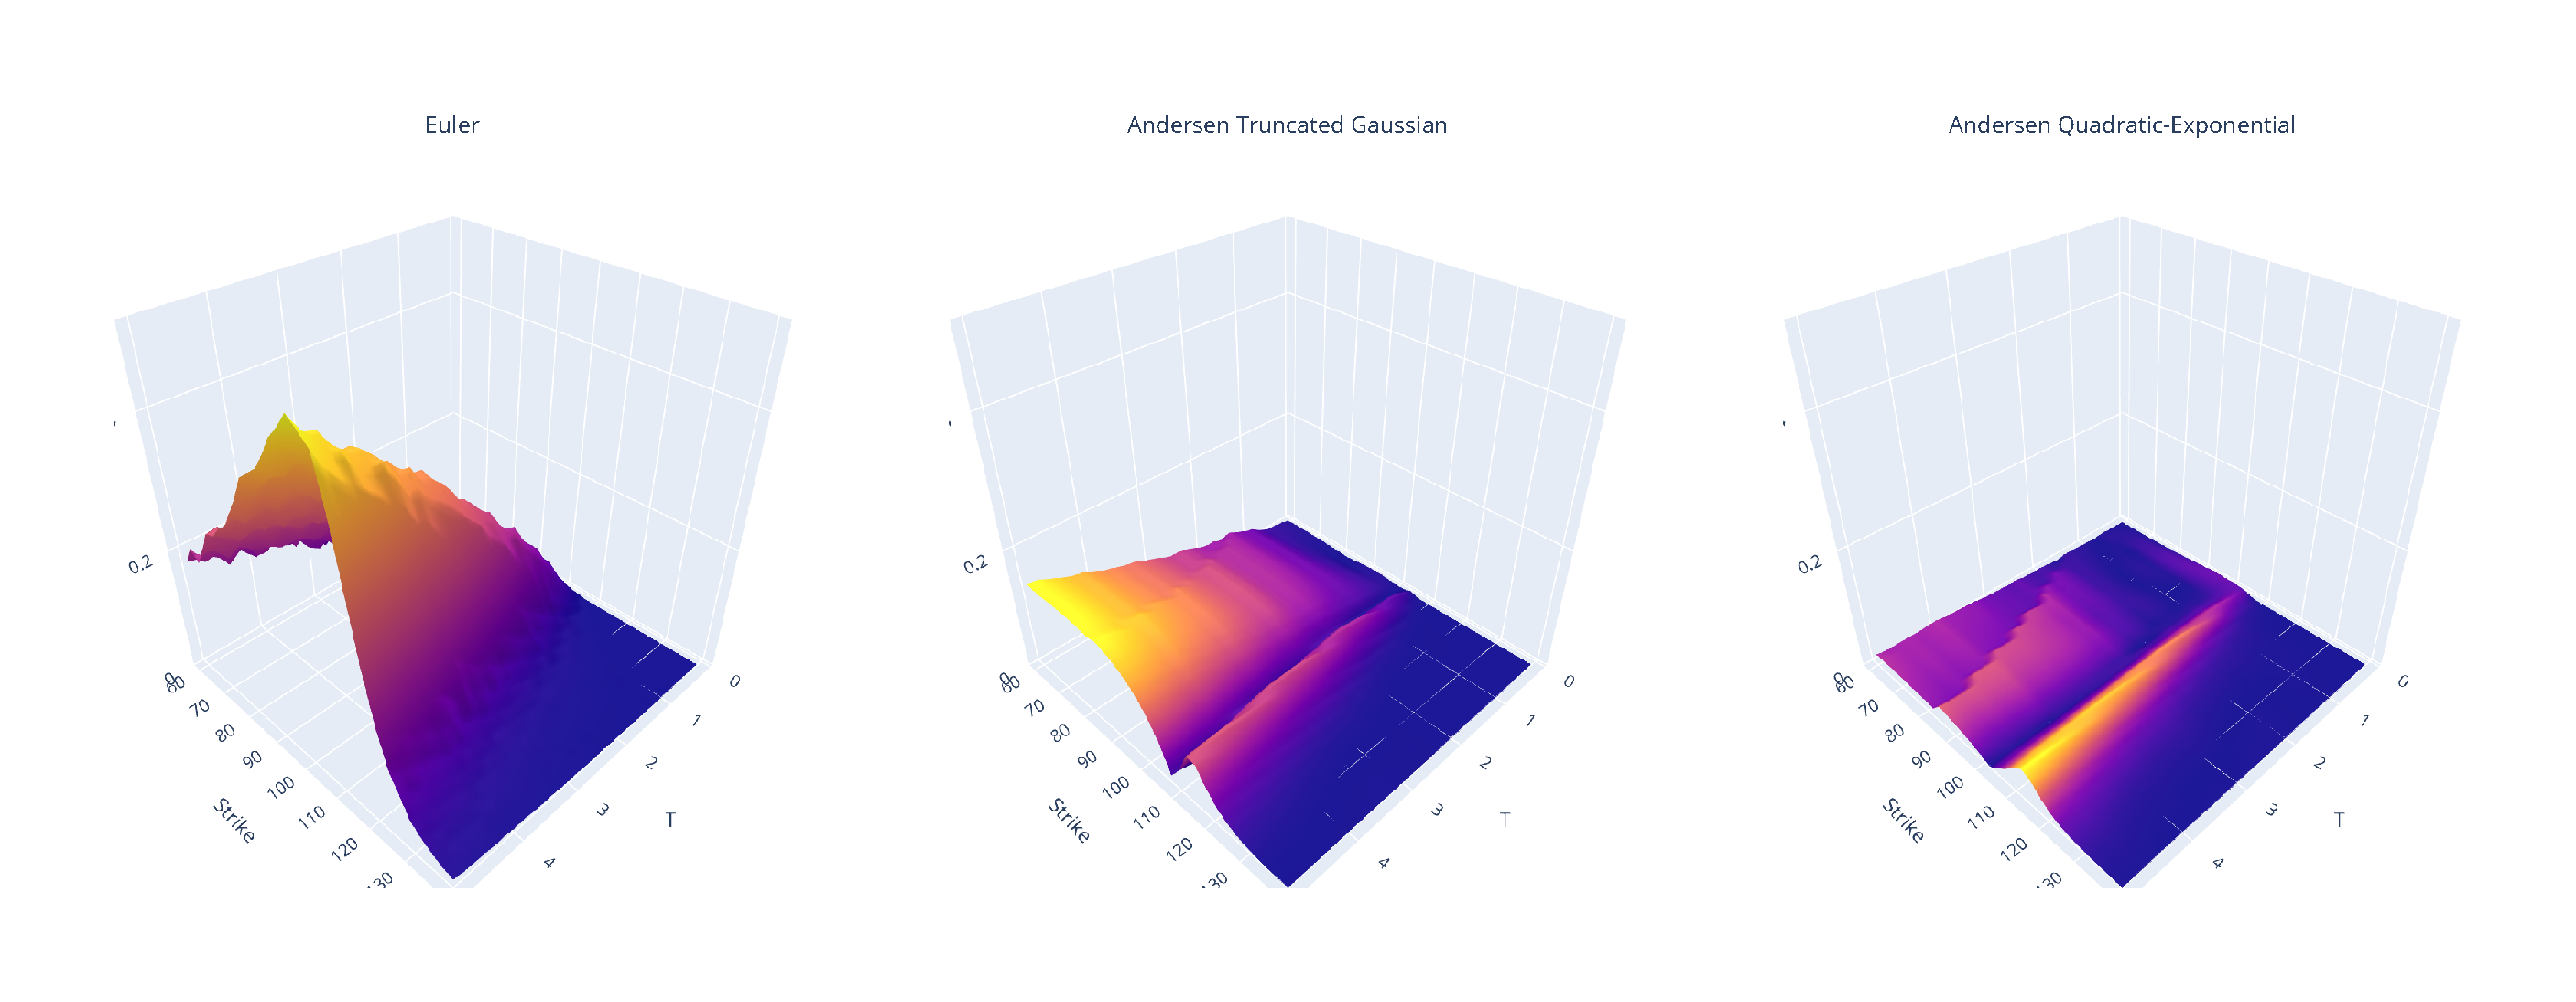
\includegraphics[width=\textwidth]{part4/pictures/err_surface_strike_T_N_T=100_param3.pdf}
        \caption{\texttt{N\_T = 100}, \texttt{absolute\_error = 5e-2}}
    \end{figure}
\end{frame}

\begin{frame}{The Surface of Errors}{Params \#4: $\kappa = 0.3$, $\gamma = 0.9$, $\rho = -0.5$, $\bar v = 0.04$, $v_0 = 0.04$}
    \begin{figure}
        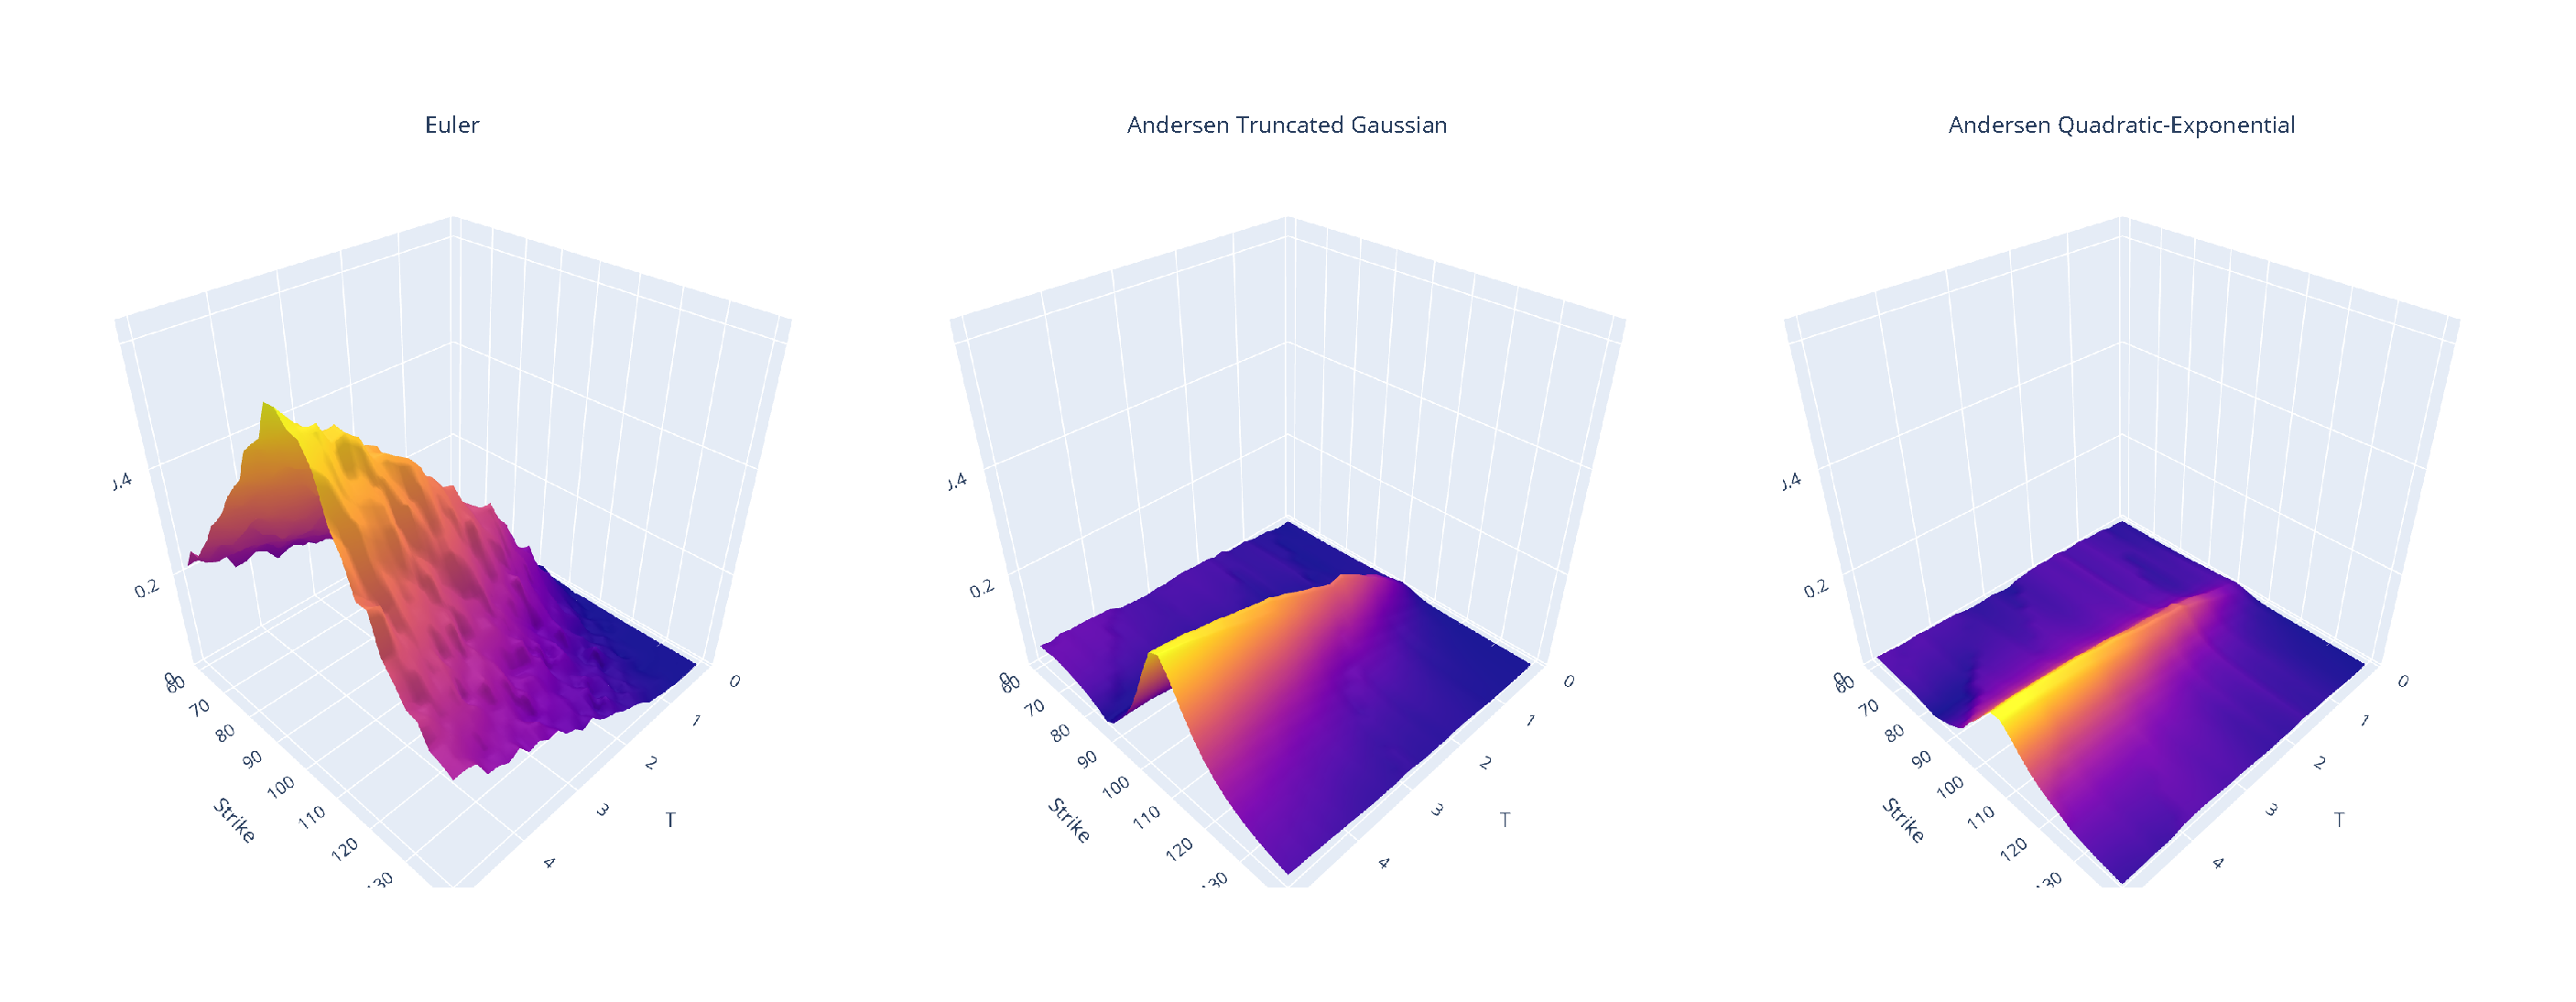
\includegraphics[width=\textwidth]{part4/pictures/err_surface_strike_T_N_T=100_param4.pdf}
        \caption{\texttt{N\_T = 100}, \texttt{absolute\_error = 5e-2}}
    \end{figure}
\end{frame}

\begin{frame}{The Surface of Errors}{Params \#5: $\kappa = 1$, $\gamma = 1$, $\rho = -0.3$, $\bar v = 0.04$, $v_0 = 0.09$}
    \begin{figure}
        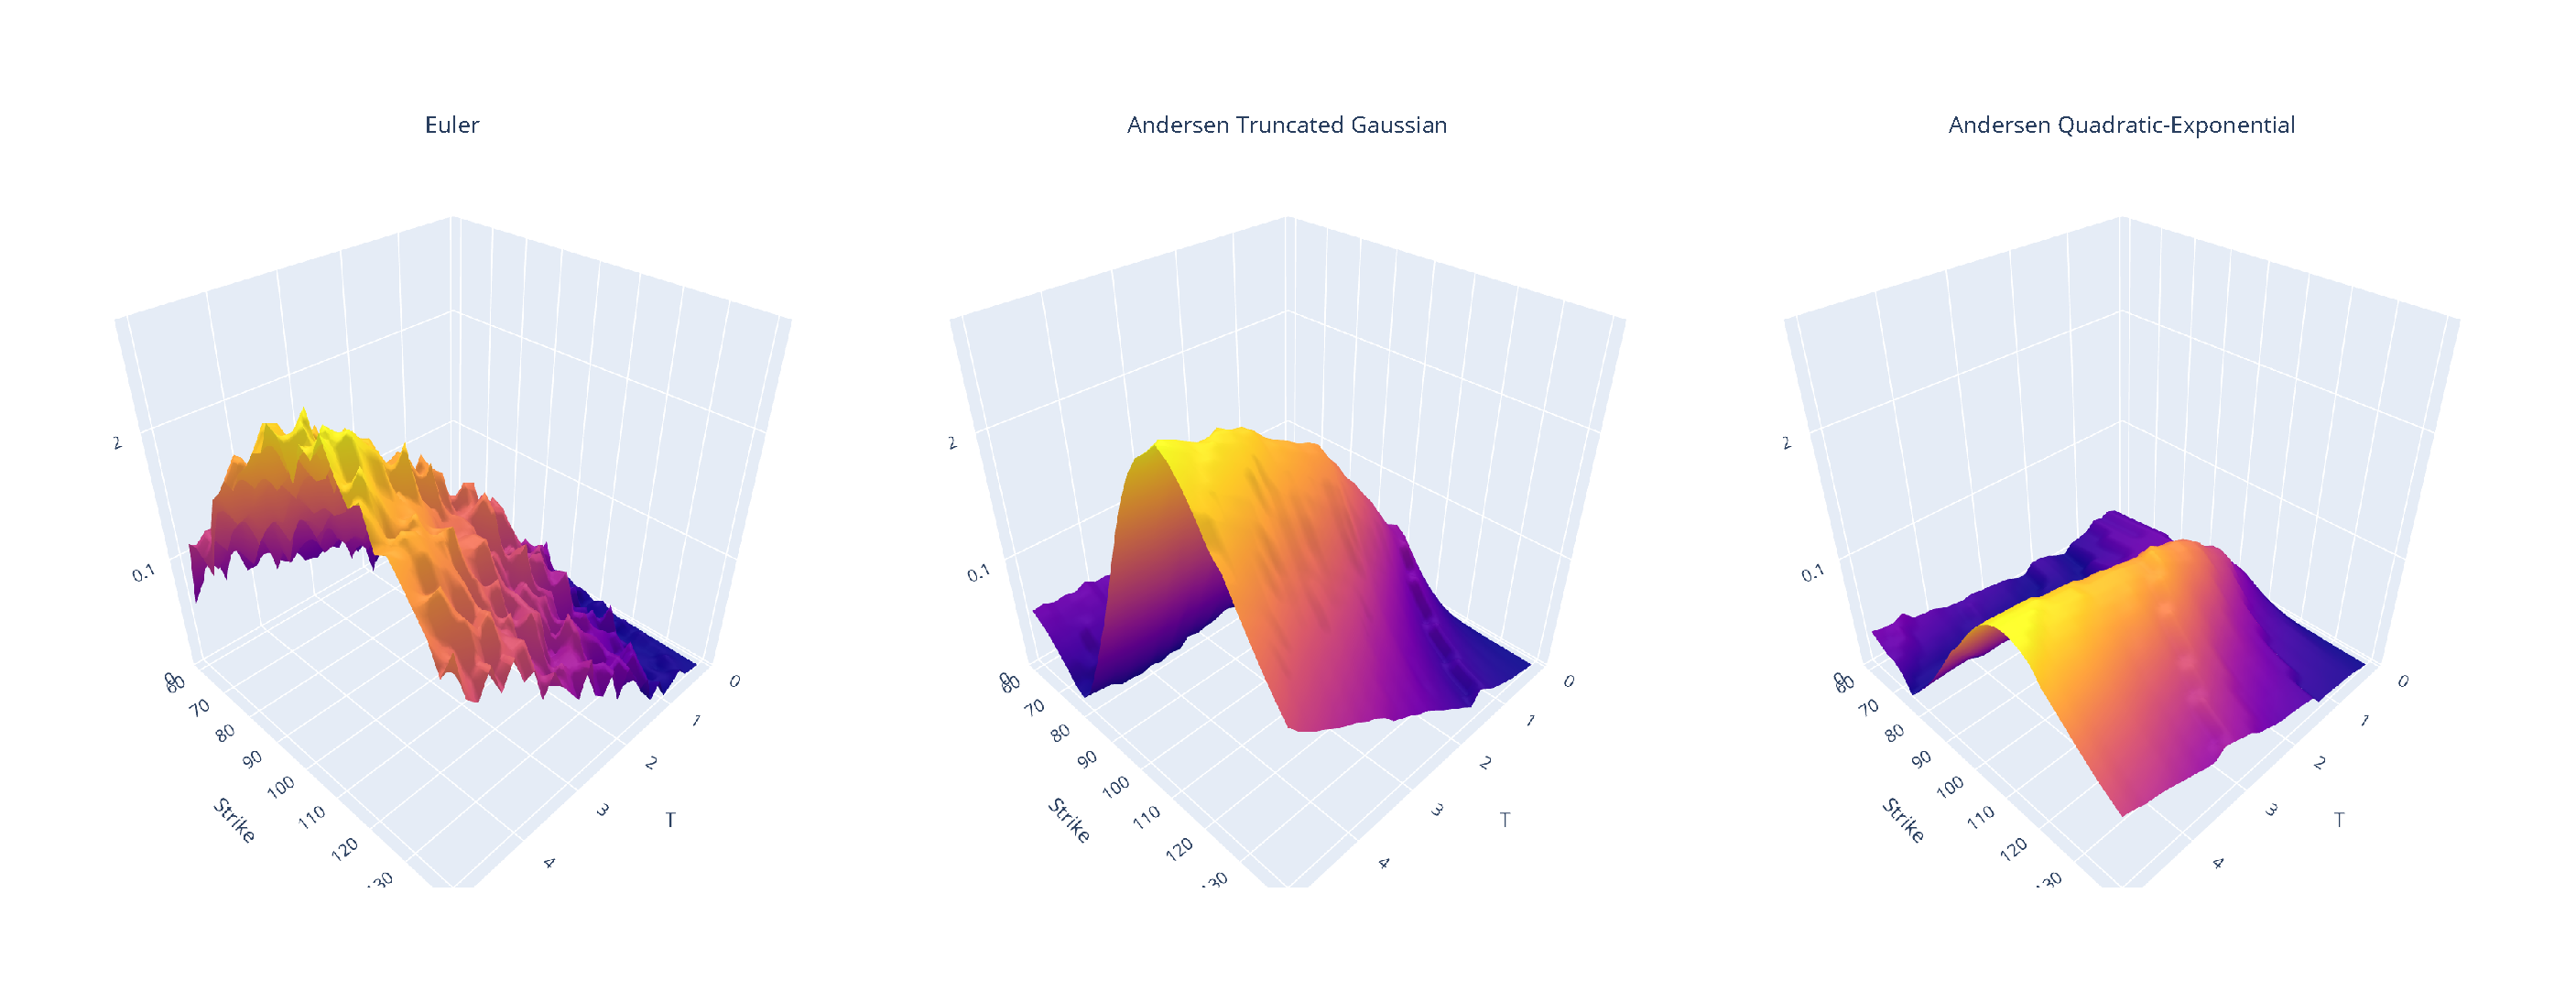
\includegraphics[width=\textwidth]{part4/pictures/err_surface_strike_T_N_T=100_param5.pdf}
        \caption{\texttt{N\_T = 100}, \texttt{absolute\_error = 5e-2}}
    \end{figure}
\end{frame}

\begin{frame}{Speed Boost compared to the Euler Scheme}{Params \#3: $\kappa = 0.5$, $\gamma = 1$, $\rho = -0.9$, $\bar v = 0.04$, $v_0 = 0.04$}
    \begin{figure}
        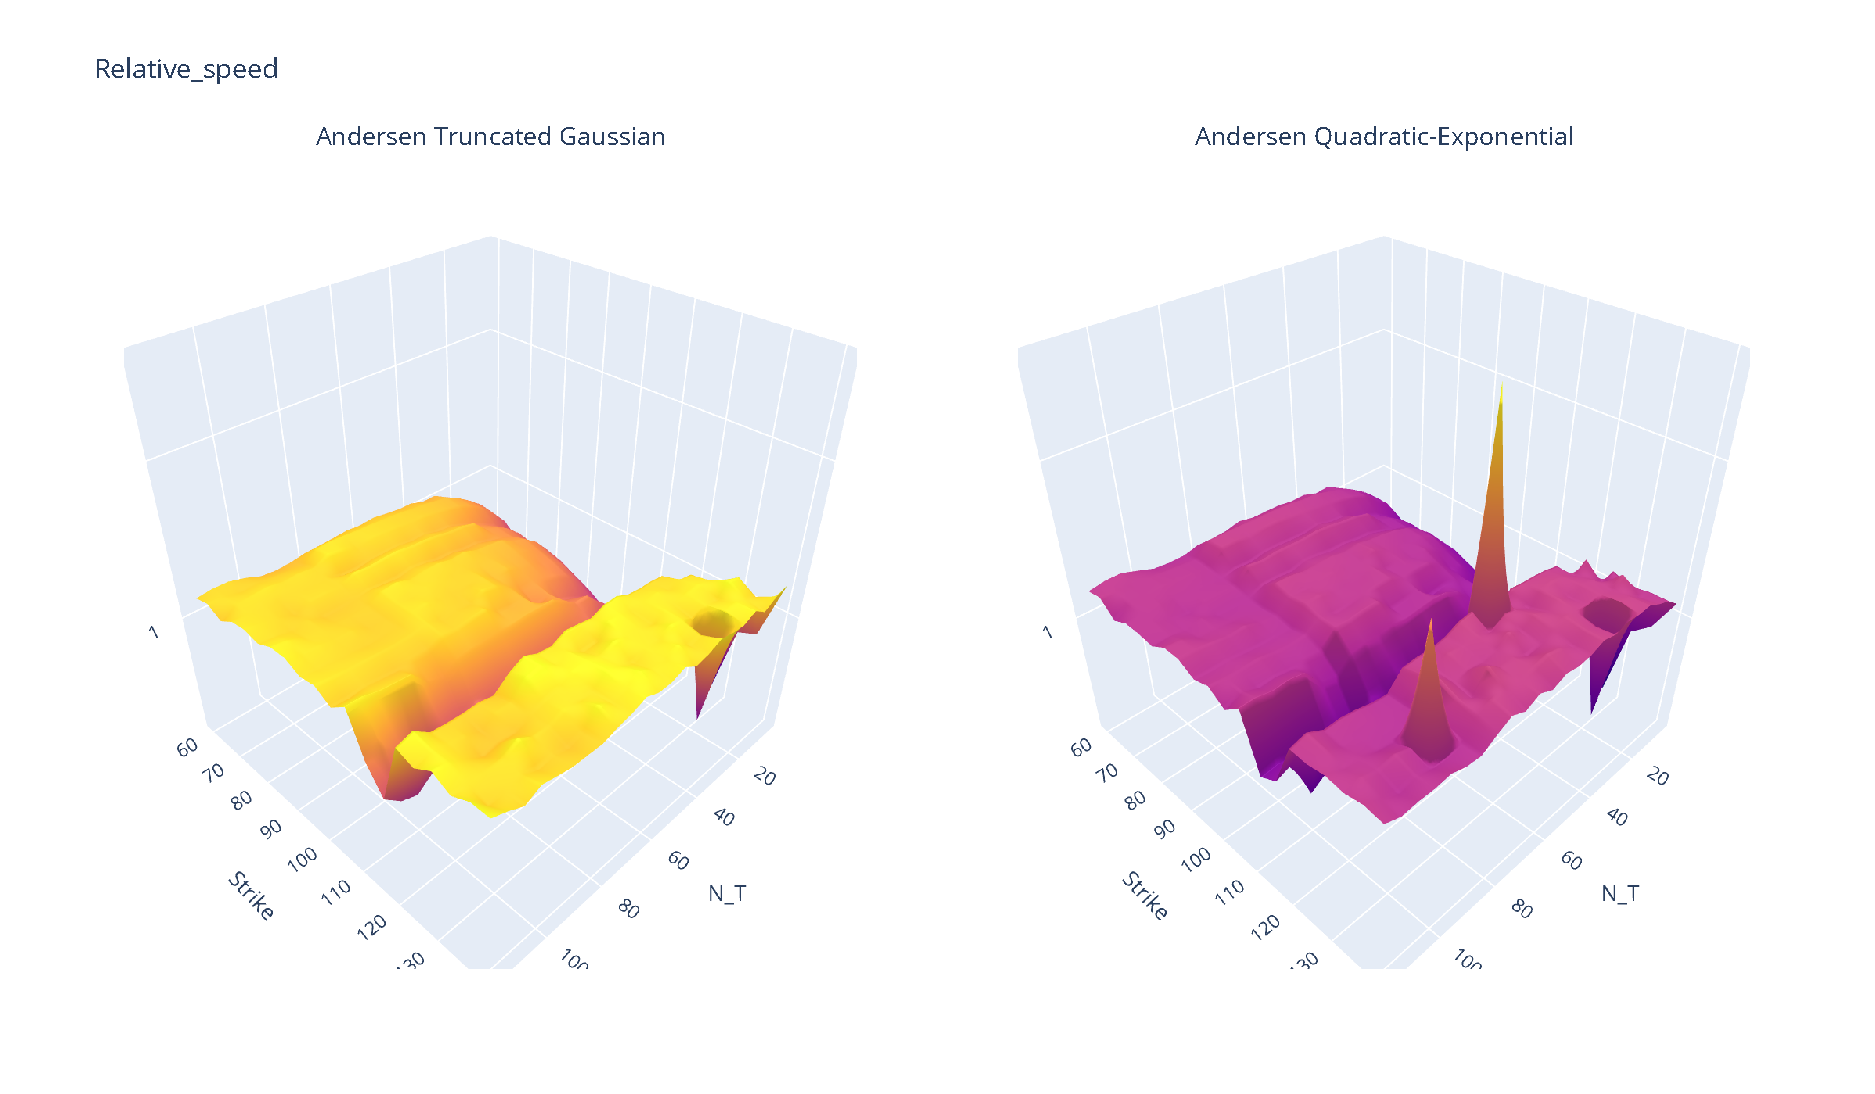
\includegraphics[width=0.9\textwidth]{part4/pictures/relative_speed_strike_N_T.pdf}
    \end{figure}
\end{frame}


